% Chapter 3

\chapter{Artefact Design \& Development} % Main chapter title
\label{Chapter3} % For referencing the chapter elsewhere, use \ref{Chapter3}
\section{Description of Artefact}
The nature of the research that is conducted in this study leads to a contrasting artefact that is delivered. The artefact is a culmination of image processing, programming, GIS data handling, and problem solving. This is made obvious as this chapter progresses further. In essence the artefact is the steps and procedures followed to come up with the final CA model.
\section{Life Cycle Methodology}
For the entire development of the Artefact a combination of three methodologies was utilised. These included:
\begin{itemize}
\item Waterfall
\item Agile
\item Scrum
\end{itemize}
The rationale for utilising this combination was due to the following factors:
\begin{itemize}
\item The emphasis on self-management for the design and development of the Artefact.
\item Incremental changes made in short iterations.
\item Segmenting problems into "chunks" and thereafter working on them in an iterative manner.
\end{itemize}
\section{Data Acquisition}
\subsection{Closed Sourced Data}
After the Literature Review was conducted the search for data began. A company by the name of GeoTerraImage (Pty) Ltd\footnote{\url{https://geoterraimage.com/}} which is located in Pretoria, South Africa was contacted and a data request was filed. The GIS data received was for an Informal settlement named \textit{"Melusi"}. The author is grateful for the data provided. The dataset received contained three main points of interest to this research:
\begin{itemize}
\item The outline or boundary of the \textit{"Melusi"} area.
\item The Land Usage in the form of housing for the year 2010 for \textit{Melusi}.
\item The Land Usage in the form of housing for the year 2020 for \textit{Melusi}.
\end{itemize}
\subsection{Open Sourced Data}
\label{sec:open}
To assist with the CA modelling additional data was needed. The following two websites  were utilised:
\begin{itemize}
\item The Humanitarian Data Exchange\footnote{\url{https://data.humdata.org/}}
\item The South African Department of Water and Sanitation\footnote{\url{https://www.dwa.gov.za/}}
\end{itemize}
From the above mentioned websites the following GIS data was acquired:
\begin{itemize}
\item All the medium-scale river coverage in South Africa.\footnote{\url{https://www.dws.gov.za/iwqs/gis_data/river/rivs500k.aspx}} This dataset was in the \texttt{.SHP} format.
\item All the Road networks in South Africa provided by HOTOSM (Humanitarian OpenStreetMap Team) and available for download by HDX (The Humanitarian Data Exchange).\footnote{\url{https://data.humdata.org/dataset/hotosm_zaf_roads}} This dataset was in the \texttt{.SHP} format.
\item High Resolution Population Density Maps \& Demographic Estimates in South Africa in the year 2019 which was once again made available for download by HDX.\footnote{\url{https://data.humdata.org/dataset/cbfc4206-35c8-42d4-a096-b2dd0aec983d}} This dataset was in the \texttt{.TIF} format.
\end{itemize}
\section{Data Exploration and Preprocessing}
\subsection{Usage of Geographic Information Systems}
\label{sec:GIS}
The use of Geographic Information Systems (GIS) was not greatly successful in this research. The factors limiting the usage were; the lack of packages, libraries, add-ons, or plug-ins that function "out-of-the-box", the ones that do work tend to fulfill niched application or specific problems.

Additional issues encountered were as follows:
\begin{itemize}
\item Incompatibility of Operating Systems.
\item GIS data formats were incompatible.
\item Researchers publising their Masters or Doctorates research made custom tools that were specific to their research.
\end{itemize}
The following GIS tools were utilised in the early stages of the research:
\begin{itemize}
\item ESRI's ArcGIS (Proprietary commercial software).\footnote{\url{https://www.esri.com/en-us/home}}
\item QGIS (Open-source software).\footnote{\url{https://qgis.org/en/site/}}
\end{itemize}

The following packages, libraries, add-ons, or plug-ins were also utilised in the early stages of the research:
\begin{itemize}
\item MOLUSCE - A plugin for QGIS for Land Use Change Evaluation.\footnote{\url{https://wiki.gis-lab.info/w/Landscape_change_analysis_with_MOLUSCE_-_methods_and_algorithms}}
\item TerraME - A Multiparadigm Modeling Toolkit.\footnote{\url{http://www.terrame.org/doku.php}}
\item GeoSOS (Geographic Simulation \& Optimization System) - A standalone program or as an add-on for ArcGIS.\footnote{\url{https://www.geosimulation.cn/GeoSOS/}}
\end{itemize}
These endeavours were also unfruitful with the reasons being the same as mentioned above.

It should be noted that the above packages do have CA modelling capabilities but were limited. The author embarked on creating his own model.

Lastly, another key hurdle was the availability of some tools which required the use of programming languages that were out of the scope of this author's skill set.

The dataset that were acquired up until this point had to analysed, therefore the next logical step was to load the GIS data into the GIS software to provide a quick overview.
\subsection{Handling of GIS Data in GIS Software}
The datasets were loaded first into ArcGIS and thereafter into QGIS. The figures below demonstrate the output achieved.
\begin{figure}[H]
\centering
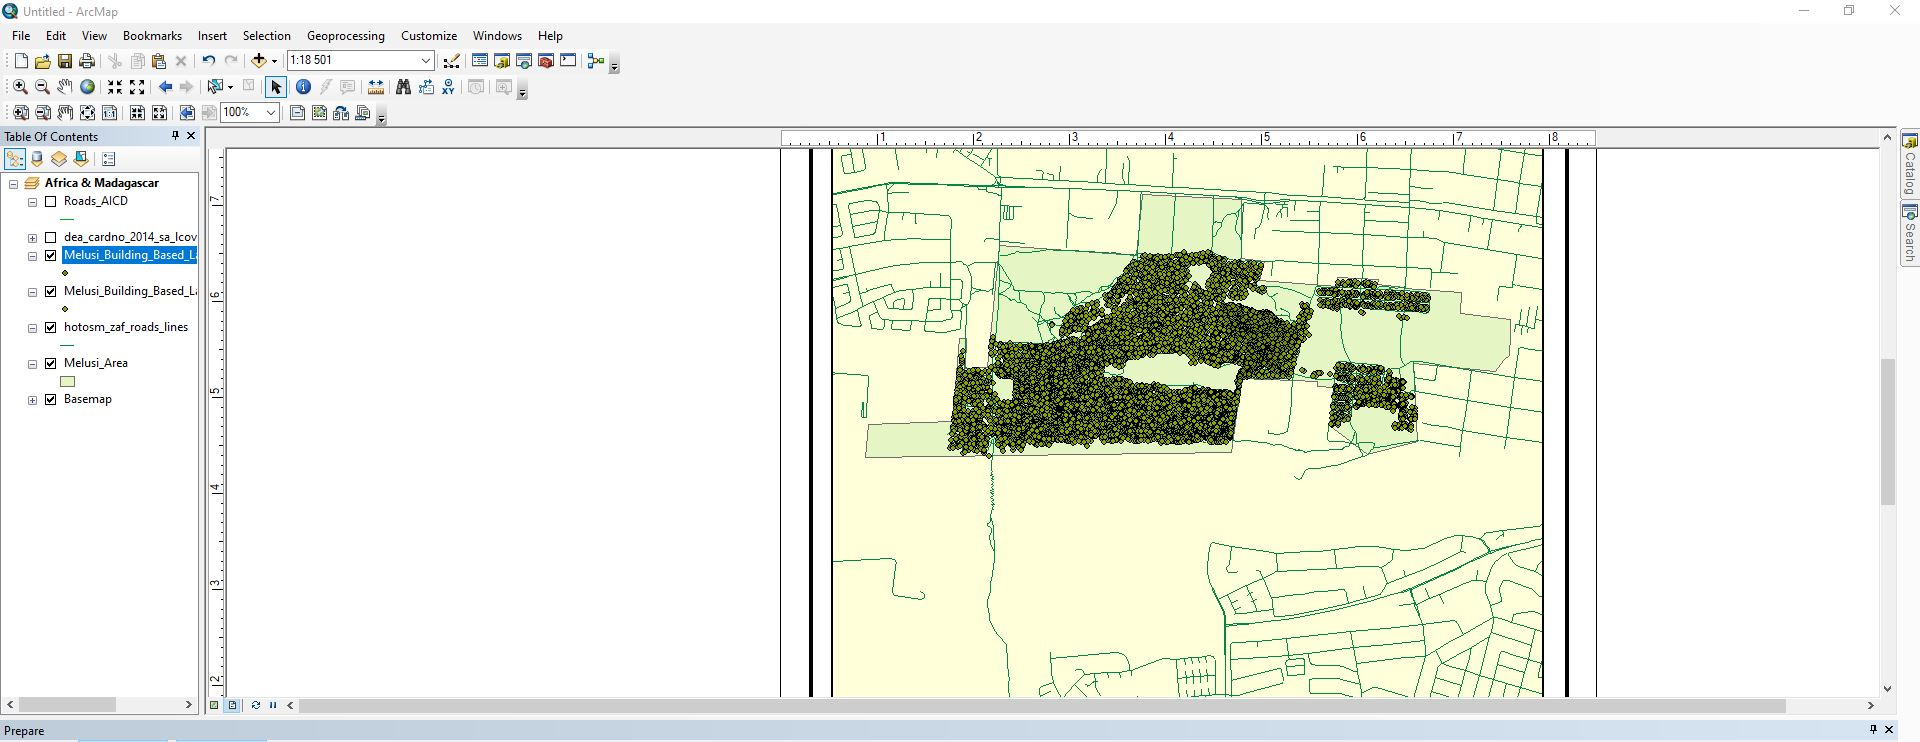
\includegraphics[scale=0.3]{Figures/Chapter3/ArcGIS}
\caption{Output of the datasets in ArcGIS}
\label{fig:Arc}
\end{figure}
\begin{figure}[H]
\centering
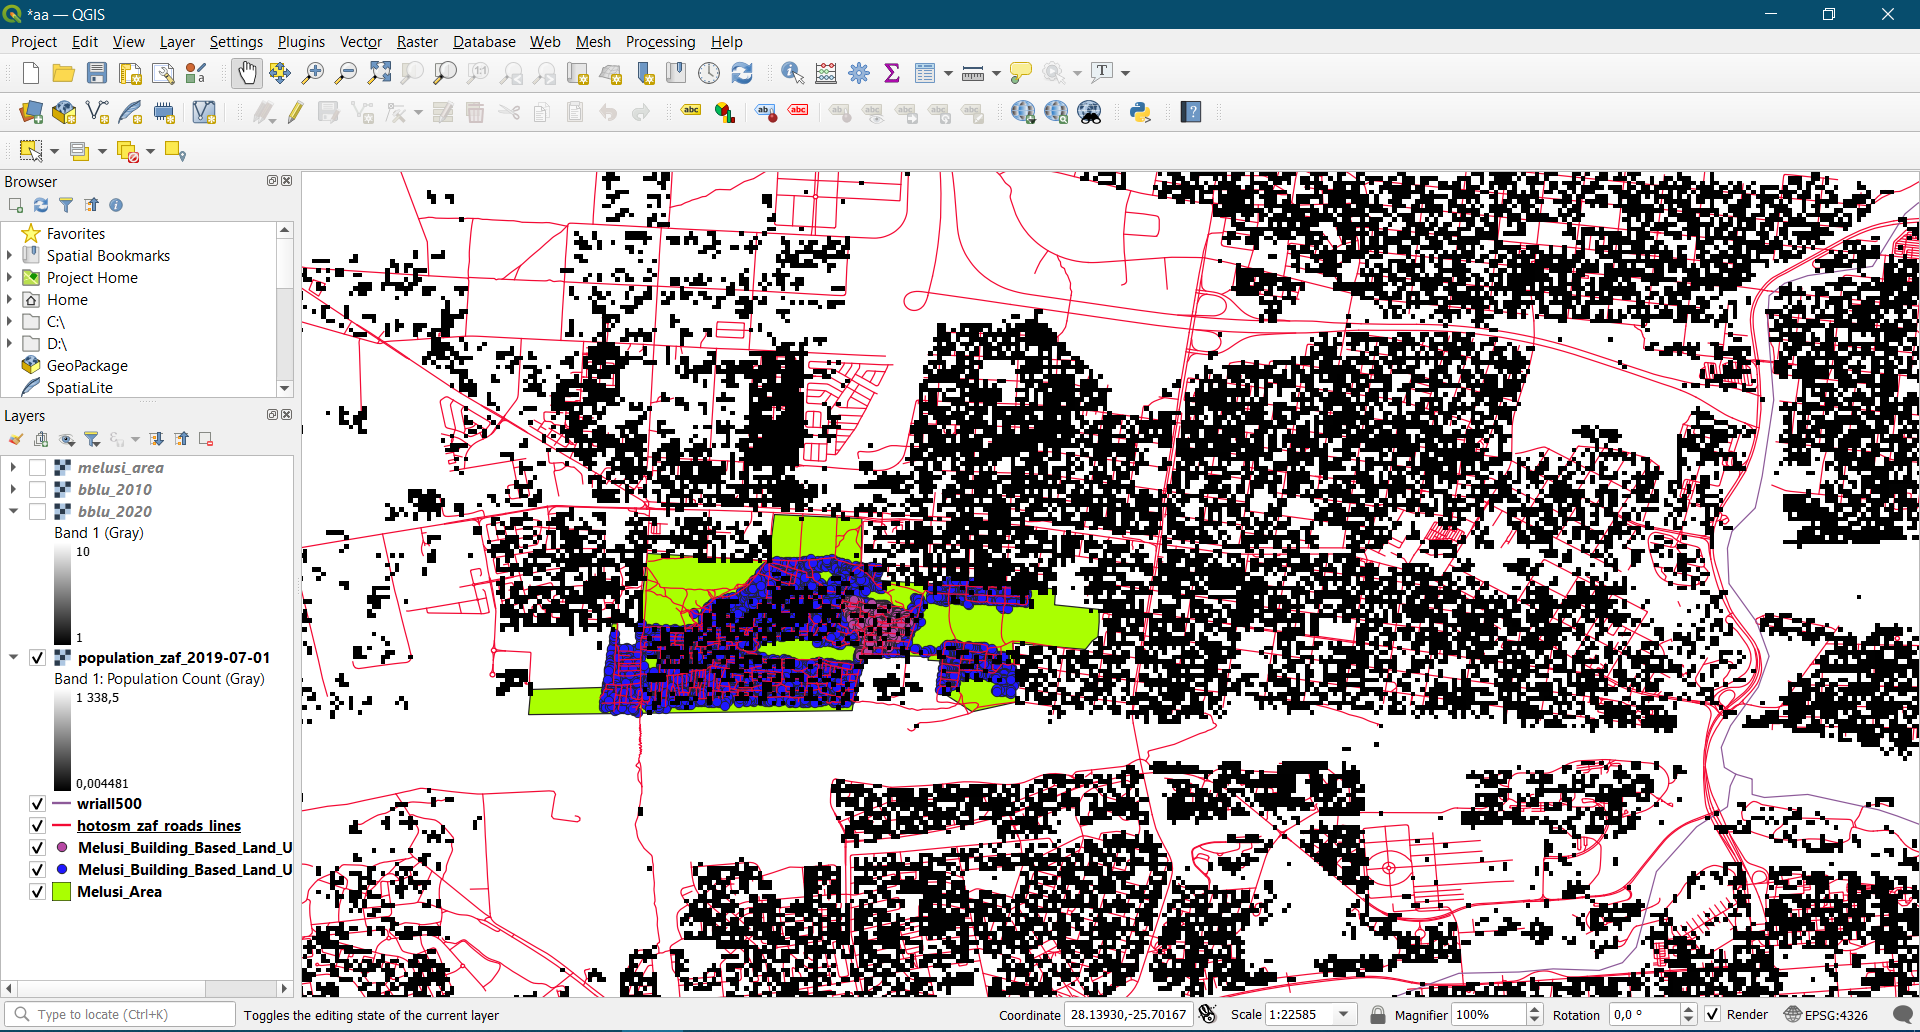
\includegraphics[scale=0.35]{Figures/Chapter3/QGIS}
\caption{Output of the datasets in QGIS}
\label{fig:Q}
\end{figure}
In the Figure \ref{fig:Arc} where ArcGIS is shown, the dark green colour represent Land Usage in the year 2020, however the Land Usage for the year 2010 was blended inside the bigger Land Usage of 2020. The lighter green colour represents the roads network in the year 2019.

In the next Figure \ref{fig:Q} where QGIS is shown, the black colour represents the population dataset, the light green colour represents the boundary of the \textit{Melusi} area. The blue colour represents the Land Usage for the year 2010, and the purple colour is the Land Usage for the year 2020. Lastly, the light pink colour represents the roads network in the year 2019.

At this juncture the dataset for the medium-scale river coverage was dropped from the research as both the GIS software indicated that there was not any rivers close by  in the area.

As was mentioned in Section \ref{sec:GIS} this was the limit of the GIS software usage in this research. The next approach was to utilise the Python programming language as well as its vast array of libraries.
\subsection{Handling of GIS Data with Python}
The primary approach used with Python was the use of Python Notebooks. These were run in two different environments:
\begin{itemize}
\item Locally using Jupyter Notebook.\footnote{\url{https://jupyter.org/}}
\item On the cloud using Google Colaboratory.\footnote{\url{https://research.google.com/colaboratory/}}
\end{itemize}
Jupyter Notebook utilises the local resources an individual has on a computer to run Python code.

Google Colab is an example of Platform as a Service (PaaS), and Infrastructure as a Service (IaaS) combined into one service.

PaaS is a cloud service model which supports application development in the cloud using languages and other tools. IaaS on the other hand is cloud service model which offers network components, storage, and processing in the cloud.\cite{pf} These service models do not require users to have powerful computing components as it is "outsourced" to these vendors such as Google.

Therefore, the only requirement for Google Colab is to utilise a modern browser that is capable of opening the Colab website to run Python code.
\\\\
The Geopandas\footnote{\url{https://geopandas.org/}} and the Matplotlib\footnote{\url{https://matplotlib.org/}} libraries were utilised to load the datasets and carry out elementary visual analysis. Additionally, the library called Folium\footnote{\url{https://python-visualization.github.io/folium/}} was utised to create an interactive map to demonstrate the boundaries of \textit{Melusi} in repect to other surrounding regions.

The first dataset to be loaded was the \textit{Melusi} dataset which had the \texttt{.SHP} files. This was done using the Geopandas \texttt{read\_file} method.\footnote{\url{https://geopandas.org/docs/reference/api/geopandas.read_file.html}}\\\\
From the Folium library the \texttt{map} method\footnote{\url{https://python-visualization.github.io/folium/modules.html\#module-folium.map}} was utilised after the coordinates were extracted from the data loaded into Geopandas and visualisations were made using Matplotlib. The \texttt{pyplot.plot} method\footnote{\url{https://matplotlib.org/stable/api/_as_gen/matplotlib.pyplot.plot.html\#matplotlib.pyplot.plot}} was used for this step.

Below are a few figures that were created in this process. The coordinates of this region can also be seen in the figures above.
For more information on these steps involved, the Appendix \ref{AppendixC} has more details.
\begin{figure}[!ht]
\centering
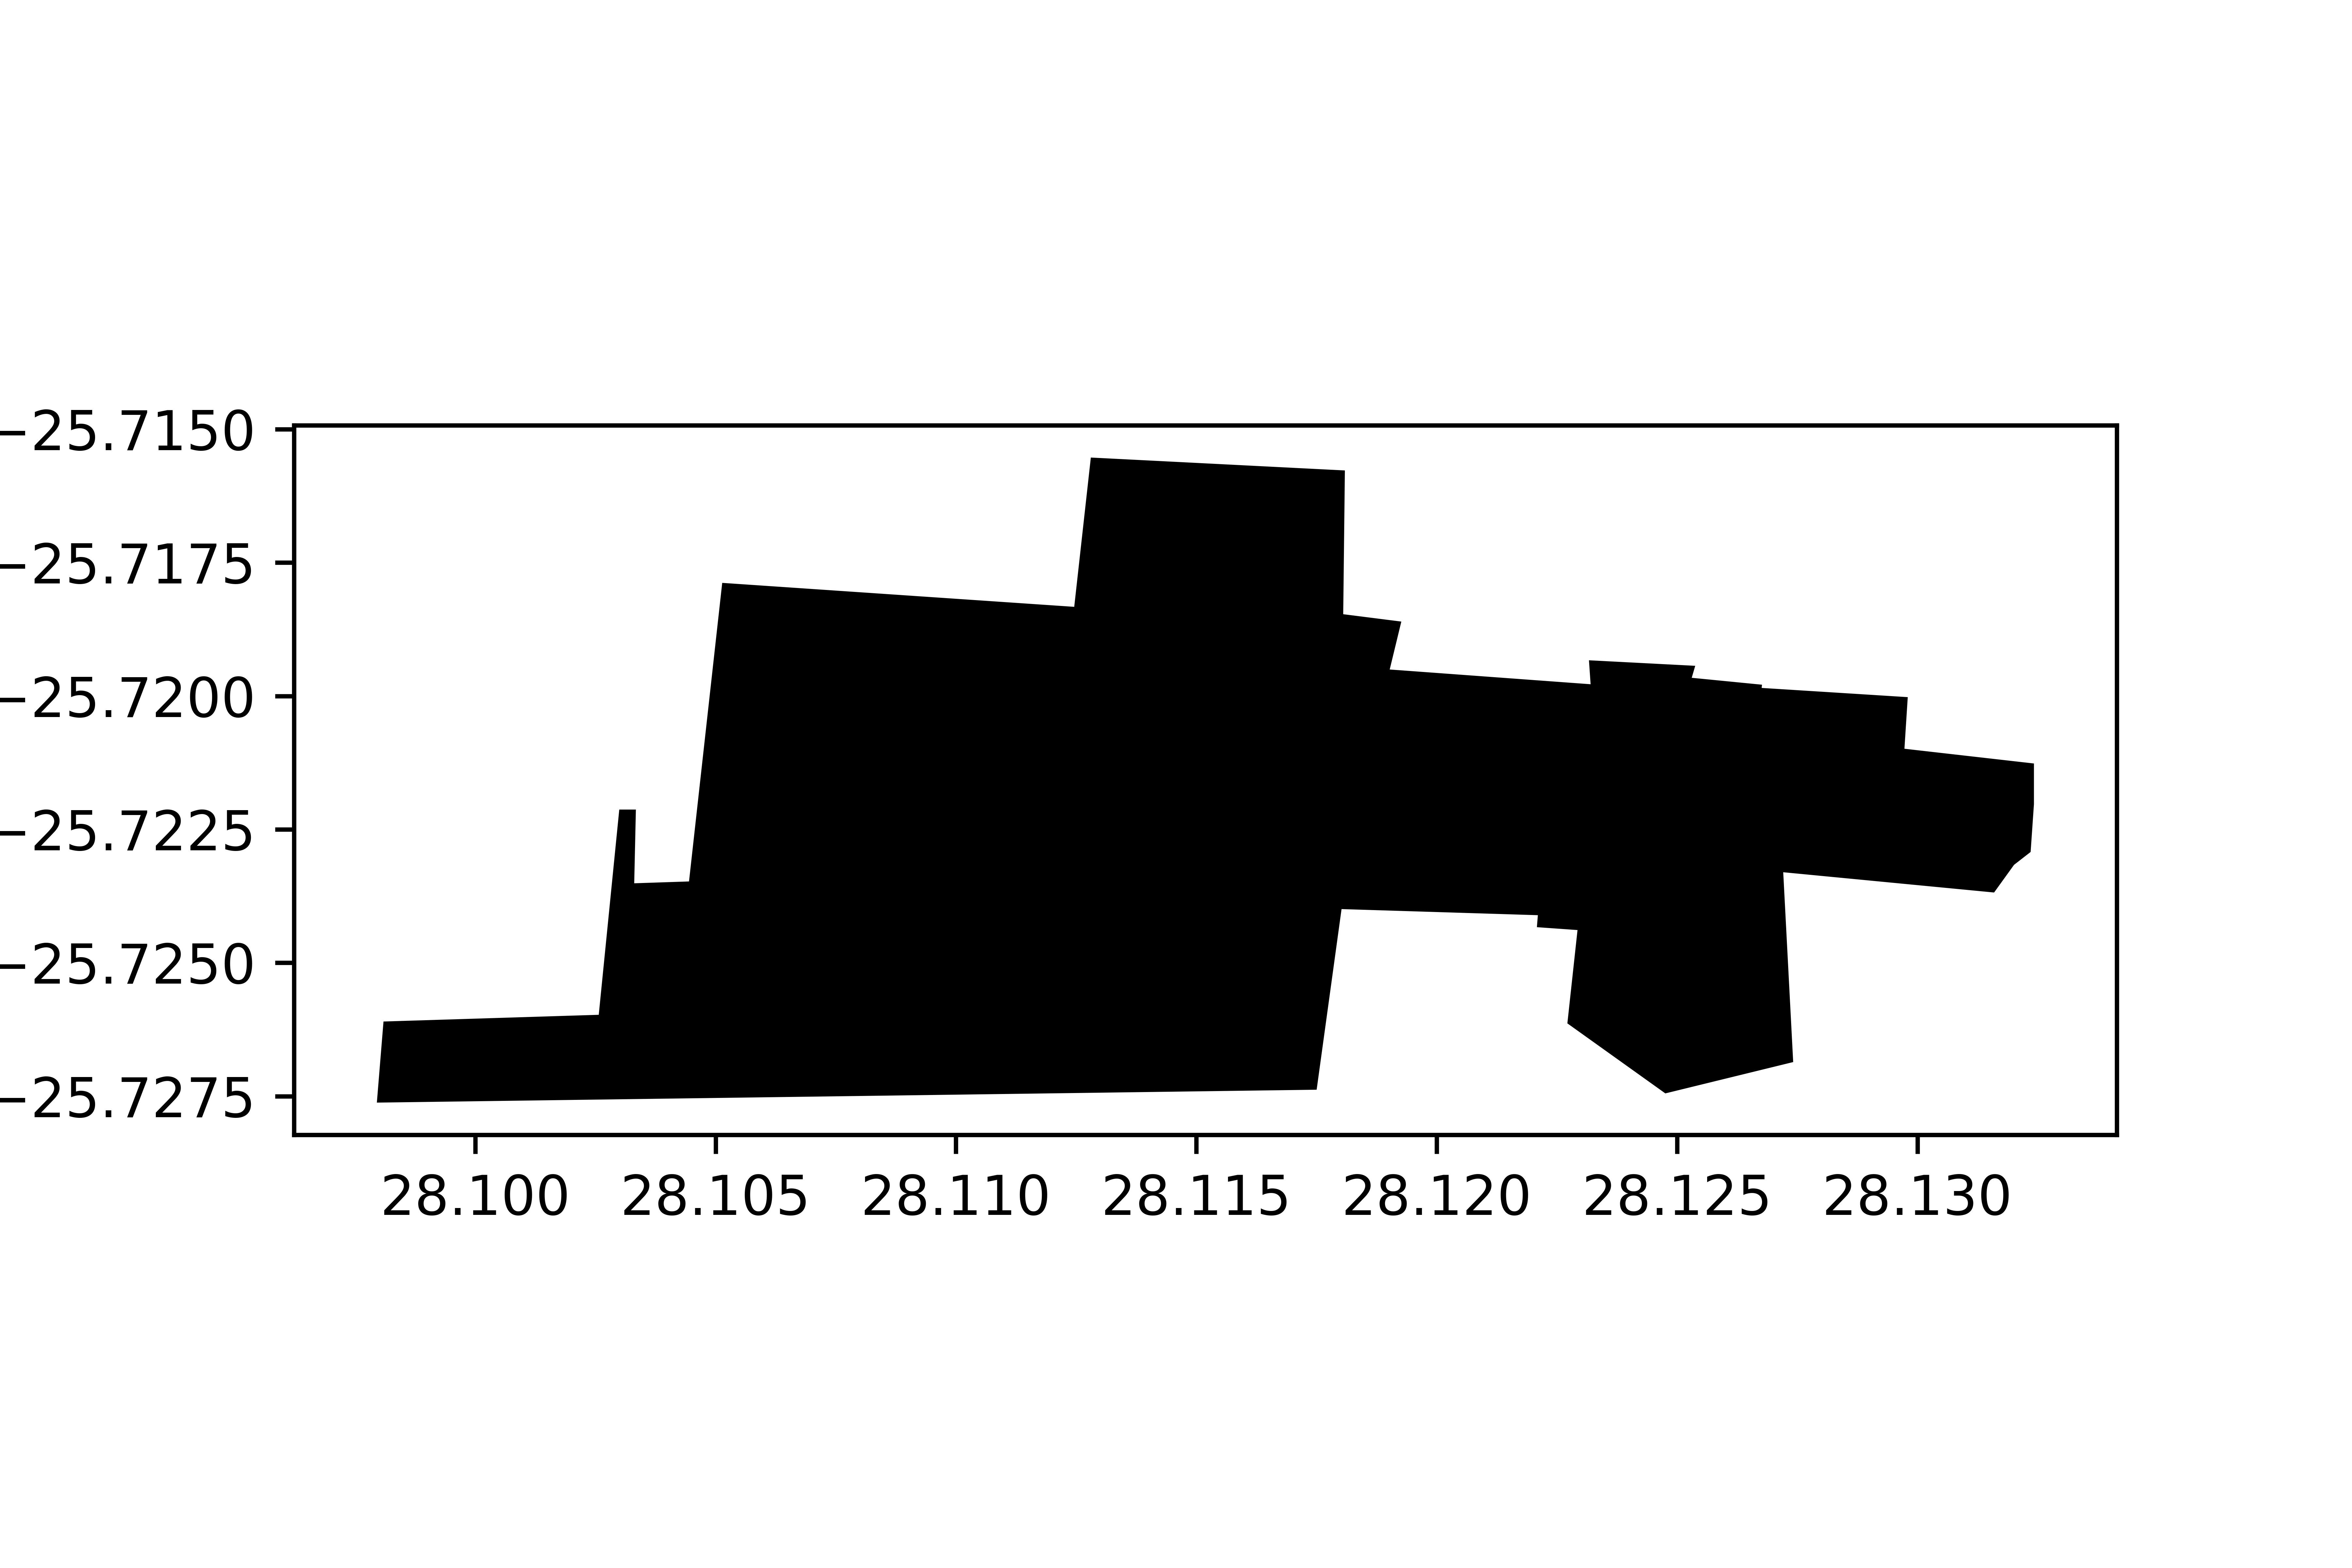
\includegraphics[width=1\textwidth]{Figures/Chapter3/MelusiArea}
\caption{The boundary of the \textit{Melusi} area}
\end{figure}
\begin{figure}[!ht]
\centering
\includegraphics[width=1\textwidth]{Figures/Chapter3/Melusi2010}
\caption{The Land Usage of the \textit{Melusi} area in 2010}
\label{fig:mel2010}
\end{figure}
\begin{figure}[!ht]
\centering
\includegraphics[width=1\textwidth]{Figures/Chapter3/Melusi2020}
\caption{The Land Usage of the \textit{Melusi} area in 2020}
\label{fig:mel2020}
\end{figure}
Once the coordinates were acquired the Folium interactive map was created of the \textit{Melusi} area. This is shown below in Figures \ref{fig:fol} and \ref{fig:fol2}. The surrounding suburbs and regions can also be seen. The webpages for these can be accessed here\footnote{\url{https://github.com/AM-ops/Hons-Project-Documentation/blob/main/Hons-Project-Documentation-Final/Web/melusi_area.html}}$^{,}$\footnote{\url{https://github.com/AM-ops/Hons-Project-Documentation/blob/main/Hons-Project-Documentation-Final/Web/melusi_area2.html}}
The file can be downloaded and thereafter viewed interactively in a browser.

The Land Usage for 2010 and 2020 can be seen in Figures \ref{fig:mel2010} and \ref{fig:mel2020}

\begin{figure}[!ht]
\centering
%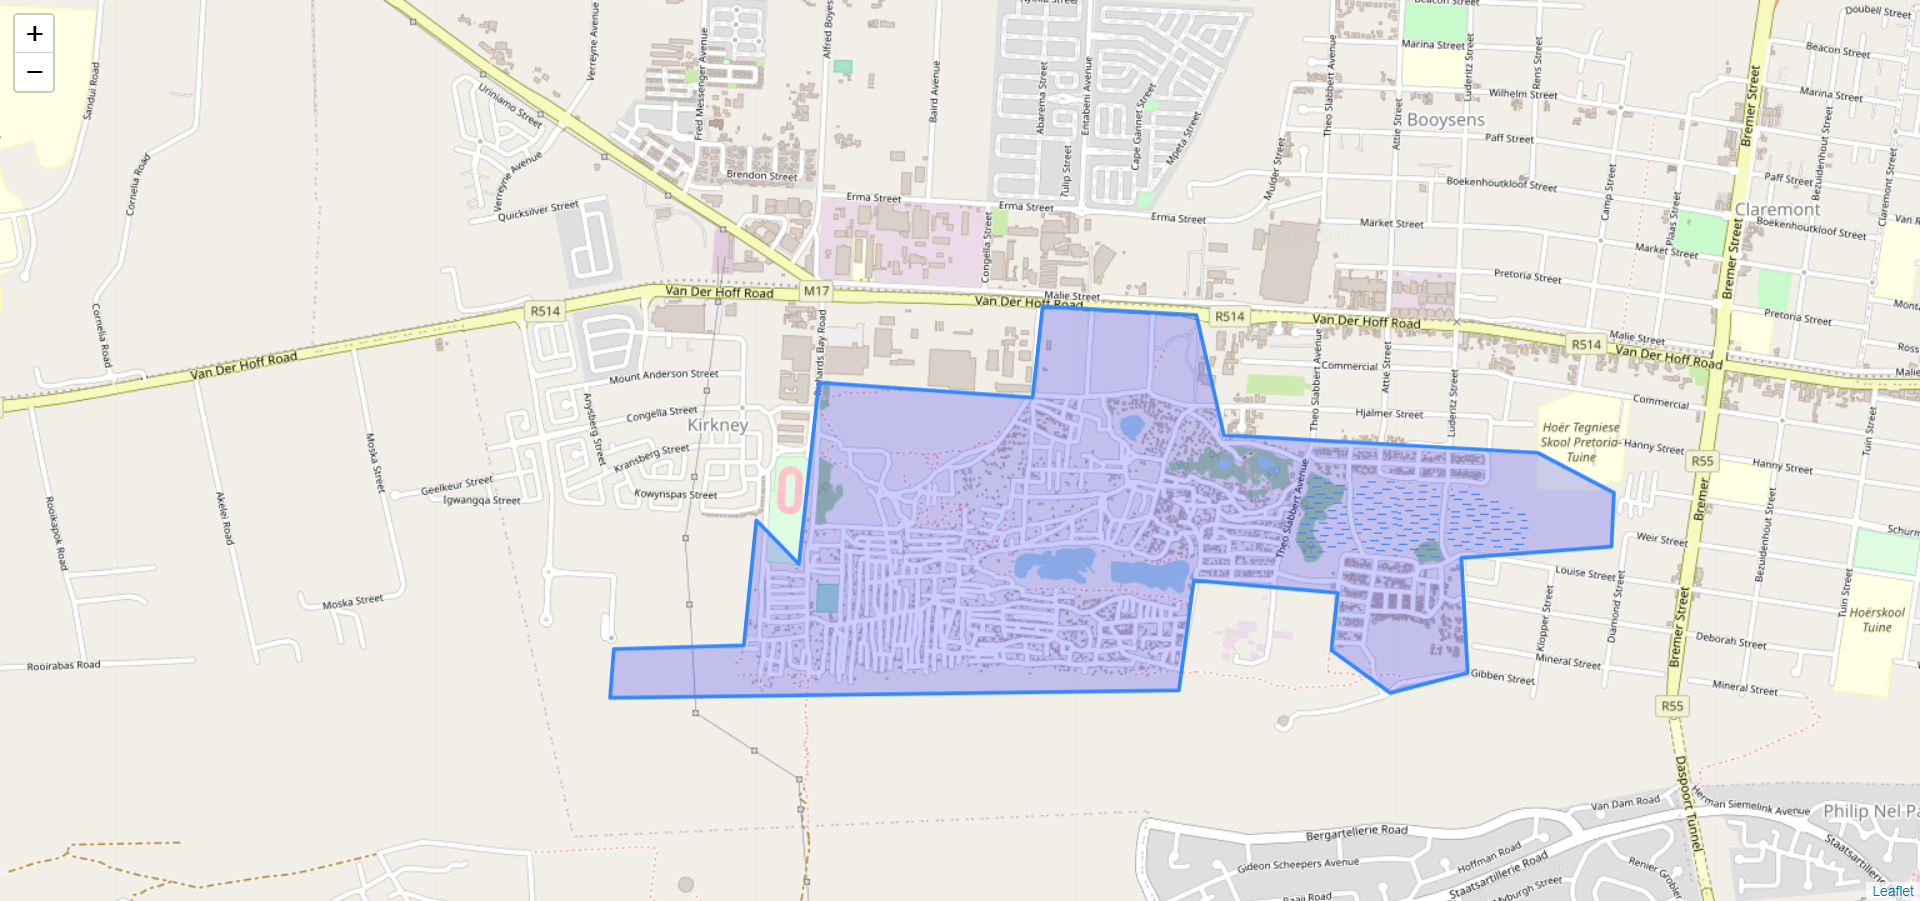
\includegraphics[width=20cm,height=15cm,keepaspectratio]{Figures/Chapter3/Folium}
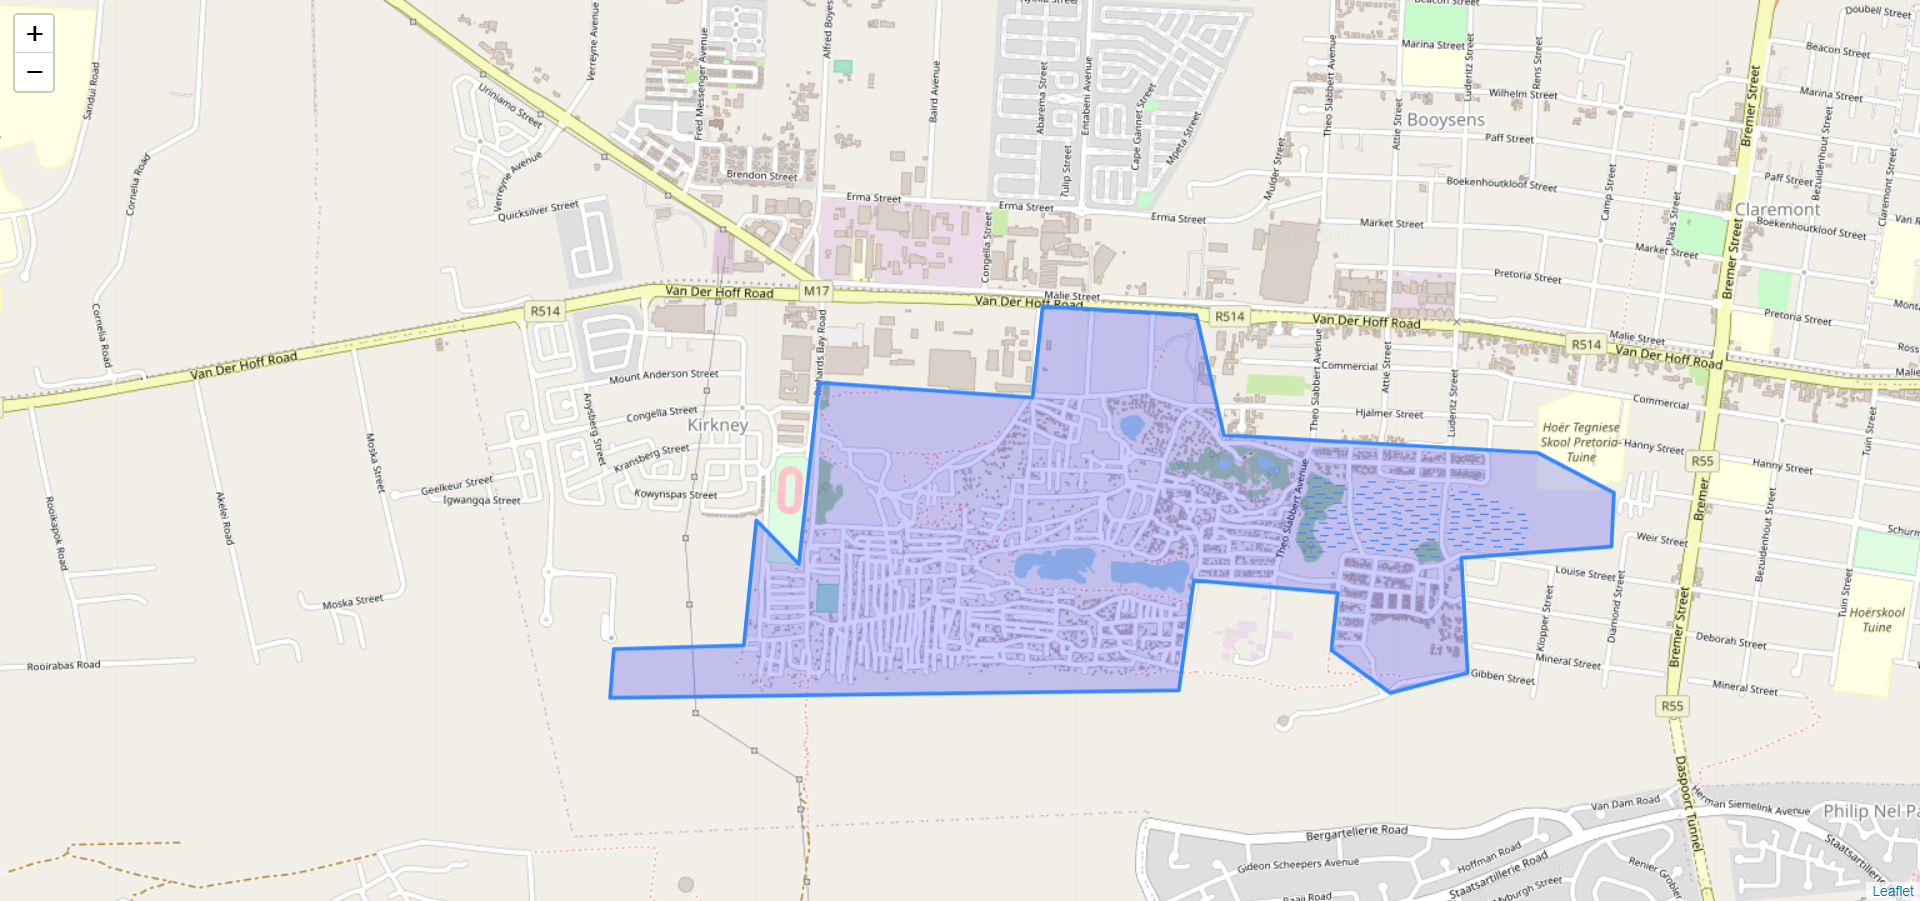
\includegraphics[scale=0.35,angle=90]{Figures/Chapter3/Folium}
\caption{Interactive map of the \textit{Melusi} area}
\label{fig:fol}
\end{figure}
\pagebreak
\begin{figure}[!ht]
\centering
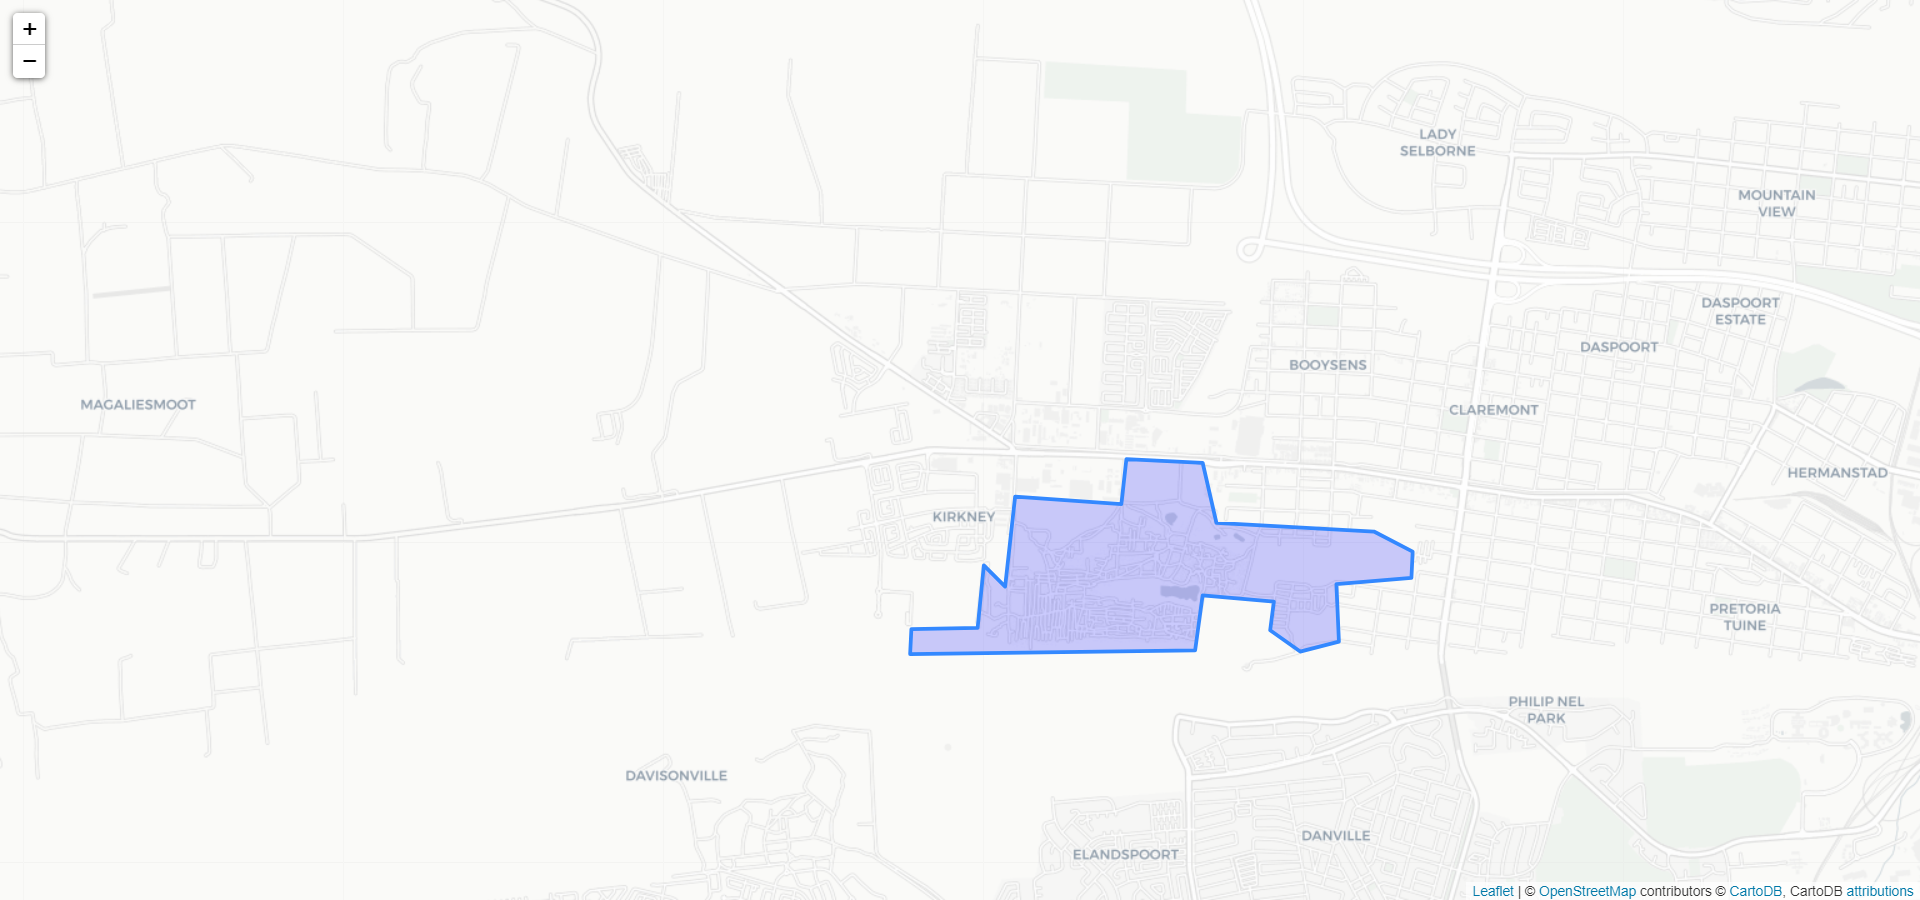
\includegraphics[scale=0.6,angle=90]{Figures/Chapter3/Folium2}
\caption{Another Interactive map of the \textit{Melusi} area}
\label{fig:fol2}
\end{figure}
After the above \textit{Melusi} area datasets were explored the next two variables needed to be explored. These were the road networks and the population datasets.

The road networks dataset as was mentioned in Section \ref{sec:open} is in the \texttt{.SHP} format, therefore once again the Geopandas \texttt{read\_file} method was employed to read the data. However the population dataset was in the \texttt{.TIF} format therefore another library Rioxarray had to be utilised.\footnote{\url{https://corteva.github.io/rioxarray/stable/rioxarray.html}} The method from this library is to read the file is \texttt{open\_rasterio}.

Data that is loaded using Geopandas is stored in \texttt{GeoDataFrames} whereas the data loaded using Rioxarray is stored in \texttt{DataArrays}. Each of these data structures have different methods and properties that allow for the manipulation of the data. This is demonstrated below.

In the next procedure the following has to be kept in mind; the aforementioned two datasets contain data for the entirety of South Africa, therefore they have to be limited to just the \textit{Melusi} area. To accomplish this firstly, the \textit{Melusi} area's boundary was extracted using the \texttt{GeoSeries.total\_bounds} property\footnote{\url{https://geopandas.readthedocs.io/en/latest/docs/reference/api/geopandas.GeoSeries.total_bounds.html}} provided by Geopandas.

Thereafter, this boundary limit was applied to the data structures mentioned earlier. This is done through the \texttt{cx} property\footnote{\url{https://geopandas.org/docs/reference/api/geopandas.GeoDataFrame.cx.html}} from Geopandas and was applied to the road networks \texttt{GeoDataFrame}. The \texttt{rio.clip\_box} method\footnote{\url{https://corteva.github.io/rioxarray/stable/_modules/rioxarray/raster_array.html\#RasterArray.clip_box}} from Rioxarray was applied to the population \texttt{DataArray}.

Matplotlib was once again employed for plotting purposes. The resulting images for the population and road networks datasets is shown in Figures \ref{fig:popgraph} and \ref{fig:roadgraph}.
\begin{figure}[H]
\centering
\includegraphics[width=1\textwidth]{Figures/Chapter3/Roads2019}
\caption{The Road Networks in the \textit{Melusi} area as of 2019}
\label{fig:roadgraph}
\end{figure}
\begin{figure}[H]
\centering
\includegraphics[width=1\textwidth]{Figures/Chapter3/Population2019}
\caption{The Population Density of the \textit{Melusi} area as of 2019}
\label{fig:popgraph}
\end{figure}
%ax = roads.plot(color="black", figsize=(7,5))
%ax.set\_axis\_off()
%ax.set(xlim=(xmin, xmax), ylim=(ymin, ymax))
%ax.autoscale\_view(scalex=False, scaley=False)
%ax.autoscale(enable=False)
%ax.autoscale(enable=False)
%plt.savefig("roads-nox.jpg",dpi=1200)
The next process involved exporting or saving high quality images of all the figures shown above namely; Figures \ref{fig:mel2010}, \ref{fig:mel2020}, \ref{fig:roadgraph}, and \ref{fig:popgraph}. A 2-Dimensional grid or lattice is needed for a CA model hence the need to export the images. An image is in essence a 2-Dimensional grid whereby the width and height is predefined and any pixel in the image can be referenced using a 2-Dimensional co-ordinate system.

The pixel density (known as Dots Per Inch or DPI)\cite{dpi} was set to 1,200 and the Matplotlib library's \texttt{pyplot.savefig}\footnote{\url{https://matplotlib.org/stable/api/_as_gen/matplotlib.pyplot.savefig.html}} method was called to save all the images. Additionally, the axes were set to be turned off\footnote{\url{https://matplotlib.org/3.1.1/api/_as_gen/matplotlib.axes.Axes.set_axis_off.html}} and, the autoscale\footnote{\url{https://matplotlib.org/3.1.1/api/_as_gen/matplotlib.pyplot.autoscale.html}} for figures was set to \texttt{False}.\\\\
Before the images were saved a few key aspects had to be verified. The first was making sure the Coordinate Reference System (CRS) was the same for all the datasets involved. The approach for \texttt{GeoDataFrames} is to call the \texttt{crs} property\footnote{\url{https://geopandas.org/docs/reference/api/geopandas.GeoDataFrame.crs.html}} and for the \texttt{DataArrays} the \texttt{rio.crs} accessor\footnote{\url{https://corteva.github.io/rioxarray/stable/getting_started/crs_management.html}} can be accessed.

The CRS for all the datasets was \textit{EPSG 4326}, therefore the process of saving the images was done immediately without the need for the CRS for any dataset to be changed.
\subsection{Image Processing with OpenCV}
\label{sec:imgproc}
After the images above were saved and analysed the following final dimensions were achieved, thanks to the high DPI;
\begin{itemize}
\item Width: 7,200 pixels
\item Height: 4,800 pixels
\end{itemize}
To assist in the CA modelling (discussed further down) and to simplify the process, one of the approached that can be taken is to scale the images (also known as resizing). Another approach is to grayscale the images. Both of these approaches were applied. The rationale behind using these approaches is as follows; A trade off can be made between computational time in modelling with the data loss in an image.\cite{impact} Additionally, the norm in Image Processing Modelling is to utilise Convolutional Neural Networks, this will not be the approach taken in this research.\cite{cnn}

With regards to grayscaling, and fields such as image recognition the method or type of algorithms utilised to grayscale color images does impact performance.\cite{gray} However in this research those finer details are not in the project scope, hence a basic grayscale operation was performed for all of the following images:
\begin{itemize}
\item Land Usage of the \textit{Melusi} area in 2010.
\item Land Usage of the \textit{Melusi} area in 2020.
\item Road networks of the \textit{Melusi} area in 2019.
\item Population Density of the \textit{Melusi} area in 2019.
\end{itemize}

The grayscale operation was carried out using the Python version of the OpenCV library\footnote{\url{https://docs.opencv.org/4.x/}}. The conversion from a RGB image to grayscale is done with the \texttt{cvtColor} method\footnote{\url{https://docs.opencv.org/3.4.15/de/d25/imgproc_color_conversions.html}}

The grayscale formula from OpenCV's Documentation is as follows:
\begin{center}
$\text{RGB[A] to Gray:} \quad Y \leftarrow 0.299 \cdot R + 0.587 \cdot G + 0.114 \cdot B$
\end{center}
Additionally, the process of scaling the images utilised the \texttt{resize} method\footnote{\url{https://docs.opencv.org/3.4.15/da/d54/group\_\_imgproc\_\_transform.html\#ga47a974309e9102f5f08231edc7e7529d}} which was called. The scale factor was $\frac{1}{3}$. This scale factor was chosen to prevent excess data. At this stage the Data Preprocessing is complete and the only aspect remaining is to to save the images after being processed. For this the \texttt{imwrite} function\footnote{\url{https://docs.opencv.org/4.x/d4/da8/group__imgcodecs.html\#gabbc7ef1aa2edfaa87772f1202d67e0ce}} from OpenCV was called for each of the four final images.

Thereafter, the Online Photo Editor, Photopea\footnote{\url{https://www.photopea.com/}} was employed to trim some of the edges of the images. The resulting dimensions of the images were as follows:
\begin{itemize}
\item Width: 2,160 pixels
\item Height: 830 pixels
\end{itemize}
These resulting dimensions were perfect for the next process which involved creating the CA model.
\subsection{Cellular Automata Modelling}
To begin the process of creating the CA model, the first step involved reading the final images created from the steps in Section \ref{sec:imgproc}. This once again required the use of OpenCV. The function employed is the \texttt{imread} function\footnote{\url{https://docs.opencv.org/4.x/d4/da8/group__imgcodecs.html\#ga288b8b3da0892bd651fce07b3bbd3a56}}.
sfsdfs \cite{imgp} Image processing

\begin{figure}[H]
\centering
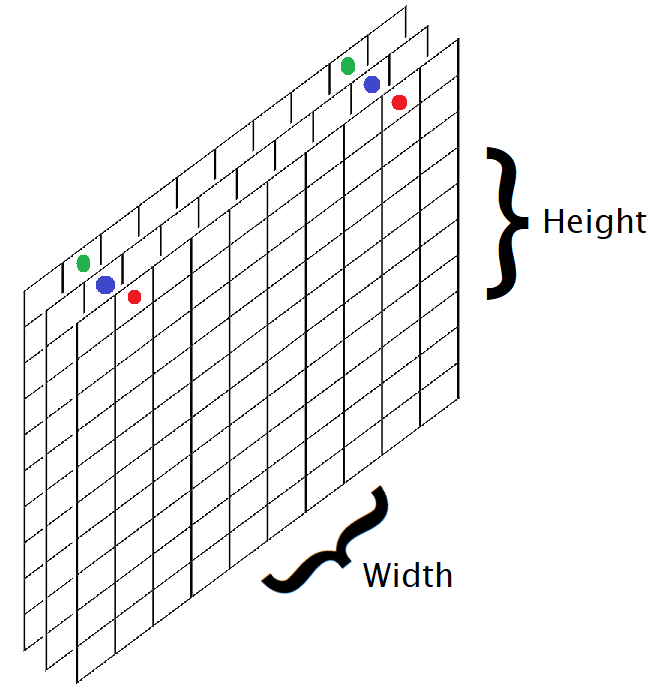
\includegraphics[width=1\textwidth]{Figures/Chapter3/gridlayers}
\caption{Numpy Arrays visualised}
\label{fig:gridlayers}
\end{figure}
